
%(BEGIN_QUESTION)
% Copyright 2010, Tony R. Kuphaldt, released under the Creative Commons Attribution License (v 1.0)
% This means you may do almost anything with this work of mine, so long as you give me proper credit

A PLC is used to count the number of cans traveling by on a conveyor belt in a fish canning factory.  An optical proximity switch detects the passage of each can, sending a discrete (on/off) signal to one of the PLC's input channels.  The PLC then counts the number of pulses to determine the number of cans that have passed by:

$$\includegraphics[width=15.5cm]{i02428x01.eps}$$

One day the canning line operator tells you the PLC has stopped counting even though cans continue to run past the proximity switch as the conveyor belt moves.  Identify what you would do to begin diagnosing this problem, justifying each step you would take.

\vskip 20pt \vbox{\hrule \hbox{\strut \vrule{} {\bf Suggestions for Socratic discussion} \vrule} \hrule}

\begin{itemize}
\item{} Identify different areas or components within this system that could possibly be at fault, as a prelude to identifying specific diagnostic steps.
\item{} Are there any ways you could diagnose this problem without the use of test equipment (e.g. multimeter)?
\item{} Explain the significance of the ``sourcing'' and ``sinking'' labels on the I/O cards as well as the proximity switch.
\end{itemize}

\underbar{file i02428}
%(END_QUESTION)





%(BEGIN_ANSWER)


%(END_ANSWER)





%(BEGIN_NOTES)

A very useful diagnostic indicator in this system is the LED indicator lamps on each PLC I/O card.  You can watch the LED on the proximity switch input to see if it blinks as cans go by.  You can also watch the ``Counter reset'' switch input to see if perhaps the reset switch is stuck on.

\vskip 20pt \vbox{\hrule \hbox{\strut \vrule{} {\bf Virtual Troubleshooting} \vrule} \hrule}

This question is a good candidate for a ``Virtual Troubleshooting'' exercise.  Presenting the diagram to students, you first imagine in your own mind a particular fault in the system.  Then, you present one or more symptoms of that fault (something noticeable by an operator or other user of the system).  Students then propose various diagnostic tests to perform on this system to identify the nature and location of the fault, as though they were technicians trying to troubleshoot the problem.  Your job is to tell them what the result(s) would be for each of the proposed diagnostic tests, documenting those results where all the students can see.

During and after the exercise, it is good to ask students follow-up questions such as:

\begin{itemize}
\item{} What does the result of the last diagnostic test tell you about the fault?
\item{} Suppose the results of the last diagnostic test were different.  What then would that result tell you about the fault?
\item{} Is the last diagnostic test the best one we could do?
\item{} What would be the ideal order of tests, to diagnose the problem in as few steps as possible?
\end{itemize}

%INDEX% PLC, troubleshooting: cannery counter system

%(END_NOTES)


